\documentclass[12 pt]{article}

\usepackage{stoversymb}
\usepackage[margin=0.75in, top=0.875in, bottom=0.875in]{geometry}
\usepackage{amsmath,amsfonts,amssymb,url,multicol,graphicx,tikz,soul}
%===makes urls render well===
\usepackage{lmodern}
\usepackage[T1]{fontenc}
%============================
\usepackage{wasysym} % smileys
\usepackage[inline]{enumitem}

\everymath{\displaystyle}

%\setenumerate{itemsep=0.25in}
\setlist[enumerate,1]{label=\arabic*., itemsep=0.5in}
\setlist[enumerate,2]{label={(\alph*)}, itemsep=0.5in}
\setlist[enumerate,3]{label={\roman*.}}
\setlist[itemize,1]{label=$\circ$, itemsep=0.25in}

\newcommand{\truefalse}[1]{#1\hfill\rule[-1mm]{220pt}{0.75pt}}
\newcommand{\hint}[1]{\vspace{3mm}\textbf{Hint}: #1}
\newcommand{\note}[1]{\textbf{Note}: #1}
\newcommand{\infsum}[3]{\sum_{{#1}={#2}}^\infty {#3}}
\newcommand{\axes}[1]{\begin{center}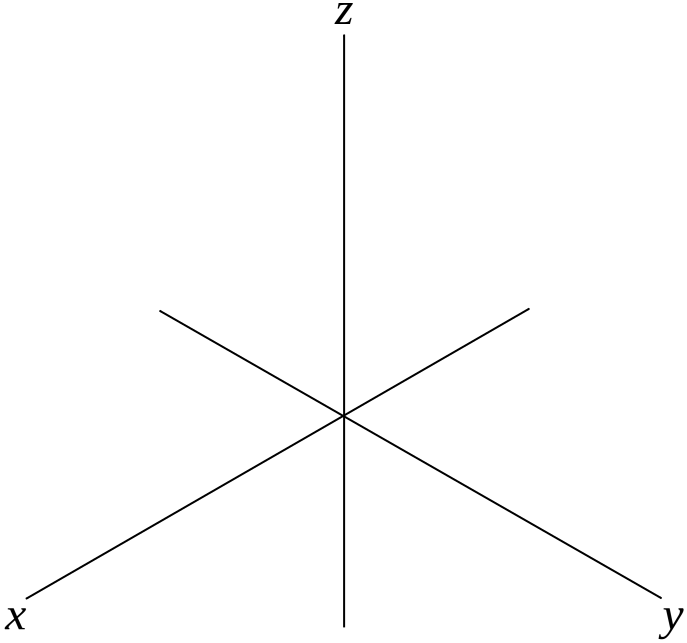
\includegraphics[scale=#1]{3DAxes}\end{center}}
\newcommand{\comps}[1]{\langle #1_1,#1_2,#1_3\rangle}
\newcommand{\compslong}[3]{\langle #1, #2, #3\rangle}
\newcommand{\ijk}[2]{#1\vect{#2}}

\graphicspath{ {./../img/} }
\DeclareGraphicsExtensions{.pdf}

\begin{document}
\begin{flushright}Name: \line(1,0){200}\end{flushright}
\begin{center}
\Large{\textbf{MAP 2302 --- Homework 1}}
\end{center}
\textbf{Directions:} Complete the following problems for a homework grade. Solutions \textit{must} be presented in a neat and professional manner in order to receive credit, answers given without showing work will not be eligible to receive partial credit, and \textit{work for the problems \textbf{must} be done on scratch paper and not on this handout!} \textbf{Date Due:} Friday, May 26.
\vspace{0.125in}
\begin{enumerate}[leftmargin=0in, rightmargin=-0.25in]
%	%========Slack==============
	\item \note{Yes, you will get graded for this question. \smiley}
	\begin{enumerate}[itemsep=0.25in]
		\item Navigate to our course homepage at
		\begin{center} \url{http://www.math.fsu.edu/~cstover/teaching/su17_map2302/}
		\end{center}
		\item Read and familiarize yourself with the three resources listed under \textit{Supplementary Resources} on the \textsc{General Info} tab.
		\item Follow the instructions for using \textsc{Slack} messenger.\begin{quote}\textbf{Note:} This may require that I approve your email address, so to avoid some last minute glitch where I don't get to your approval on-time, please don't wait to do this!\end{quote}
		\item Navigate to the channel \url{#introductions} in the left column under \textsc{Channels}; its browser URL should be something like \url{https://summer2017-ode.slack.com/messages/introductions}.
		\item Introduce yourself by answering each of the following questions:
		\begin{quote}\textbf{Note:} This will be visible to everyone who signs into our class's chat room, so you definitely want to keep these answers PG-13, safe for work, and non-incriminatory. {\Large\smiley}\end{quote}
		\begin{enumerate}[label=(\roman*),itemsep=3mm]
			\item What is your name?
			\item Where are you from (using any interpretation you'd like)?
			\item What is the best (interpret this however you'd like) place you've ever visited/lived? Why is it so special to you?
			\item How long have you been in Tallahassee?
			\item What is your major?
			\item What do you like to do for fun? (besides differential equations, of course!)
			\item What is the coolest math/science ``thing'' you know? Why is it interesting to you?
		\end{enumerate}
		\item Under which username did you register for \textsc{Slack}?\hspace{6mm}\line(1,0){200}
	\end{enumerate}

	\newpage
	
	\item For each of the following differential equations, determine whether it's separable, linear, or neither. If it's separable, separate it; if it's linear, compute its integrating factor. \textbf{Do not solve!}
	\begin{enumerate}
		\item $y''+y'=2y + \sin{x}$.
		\item $2xy'-x^2y=\sin{x}+e^x$.
		\item $y'=x^3\sin{y}$.
		\item $y'=x^3\sin{y}-y$.
		\item $y'=x^3\sin{x}-y$.
	\end{enumerate}

	\item Given the slope field below, draw the (approximate) integral curves passing through each of the indicated points.
	\begin{center}
		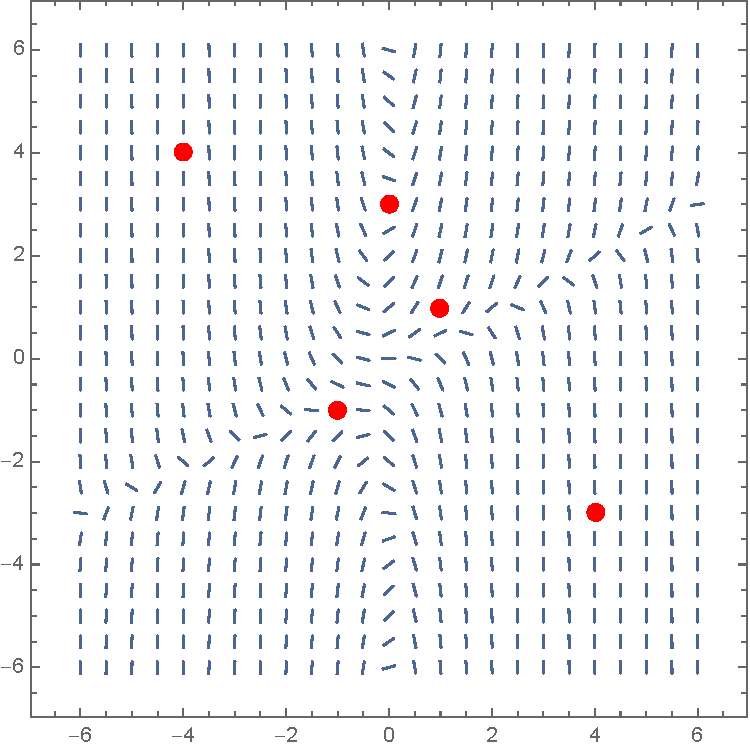
\includegraphics[scale=0.875]{hw1_slopes}
	\end{center}

	\newpage
	
	\item Each of the following questions relates to the equation $\frac{dy}{dx}=3(1+y^2)\sec^2(x)$.
	\begin{enumerate}[itemsep=1.75in]
		\item Is this ODE separable, linear, or other? How do you know?
		\item Compute the general solution for this ODE.
		\item Find the particular solution of this ODE subject to the initial condition $y(0)=1$.
		\item Determine the interval in which the solution in part (c) exists.
		
		\hint{The part of the domain of $\tan{x}$ containing $x=0$ is $(-\pi/2,\pi/2)$.}
	\end{enumerate}

	\newpage
	
	\item Each of the following questions relates to the equation $x\frac{dy}{dx}-\frac{3}{\ln{x}}\,y=2x^2\ln^3{x}$.
	\begin{enumerate}[itemsep=1.75in]
		\item Is this ODE separable, linear, or other? How do you know?
		\item Compute the general solution for this ODE. 
		
		\hint{Use $u$-substitution to find the integrating factor $m(x)$; notice that $p(x)$ has a minus sign; and watch your algebra! There's \textit{lots} of cancellation when finding $m(x)$!}.
		\item Find the particular solution of this ODE subject to the initial condition $y(e)=e+e^2$.
		\item Determine the interval in which the solution in part (c) exists. 
		
		\hint{In precalc, you learned where things like $\ln(x)$, etc., are continuous.}
	\end{enumerate}
\end{enumerate}
\end{document}